\documentclass[tikz,border=10pt]{standalone}
\usepackage[utf8]{inputenc}
\usepackage[T1]{fontenc}
\usepackage{lmodern}
\usepackage{tikz}
\usepackage{amsmath}
\usetikzlibrary{shapes.geometric, arrows.meta, positioning, calc, fit, backgrounds, decorations.pathreplacing, shadows}

\begin{document}
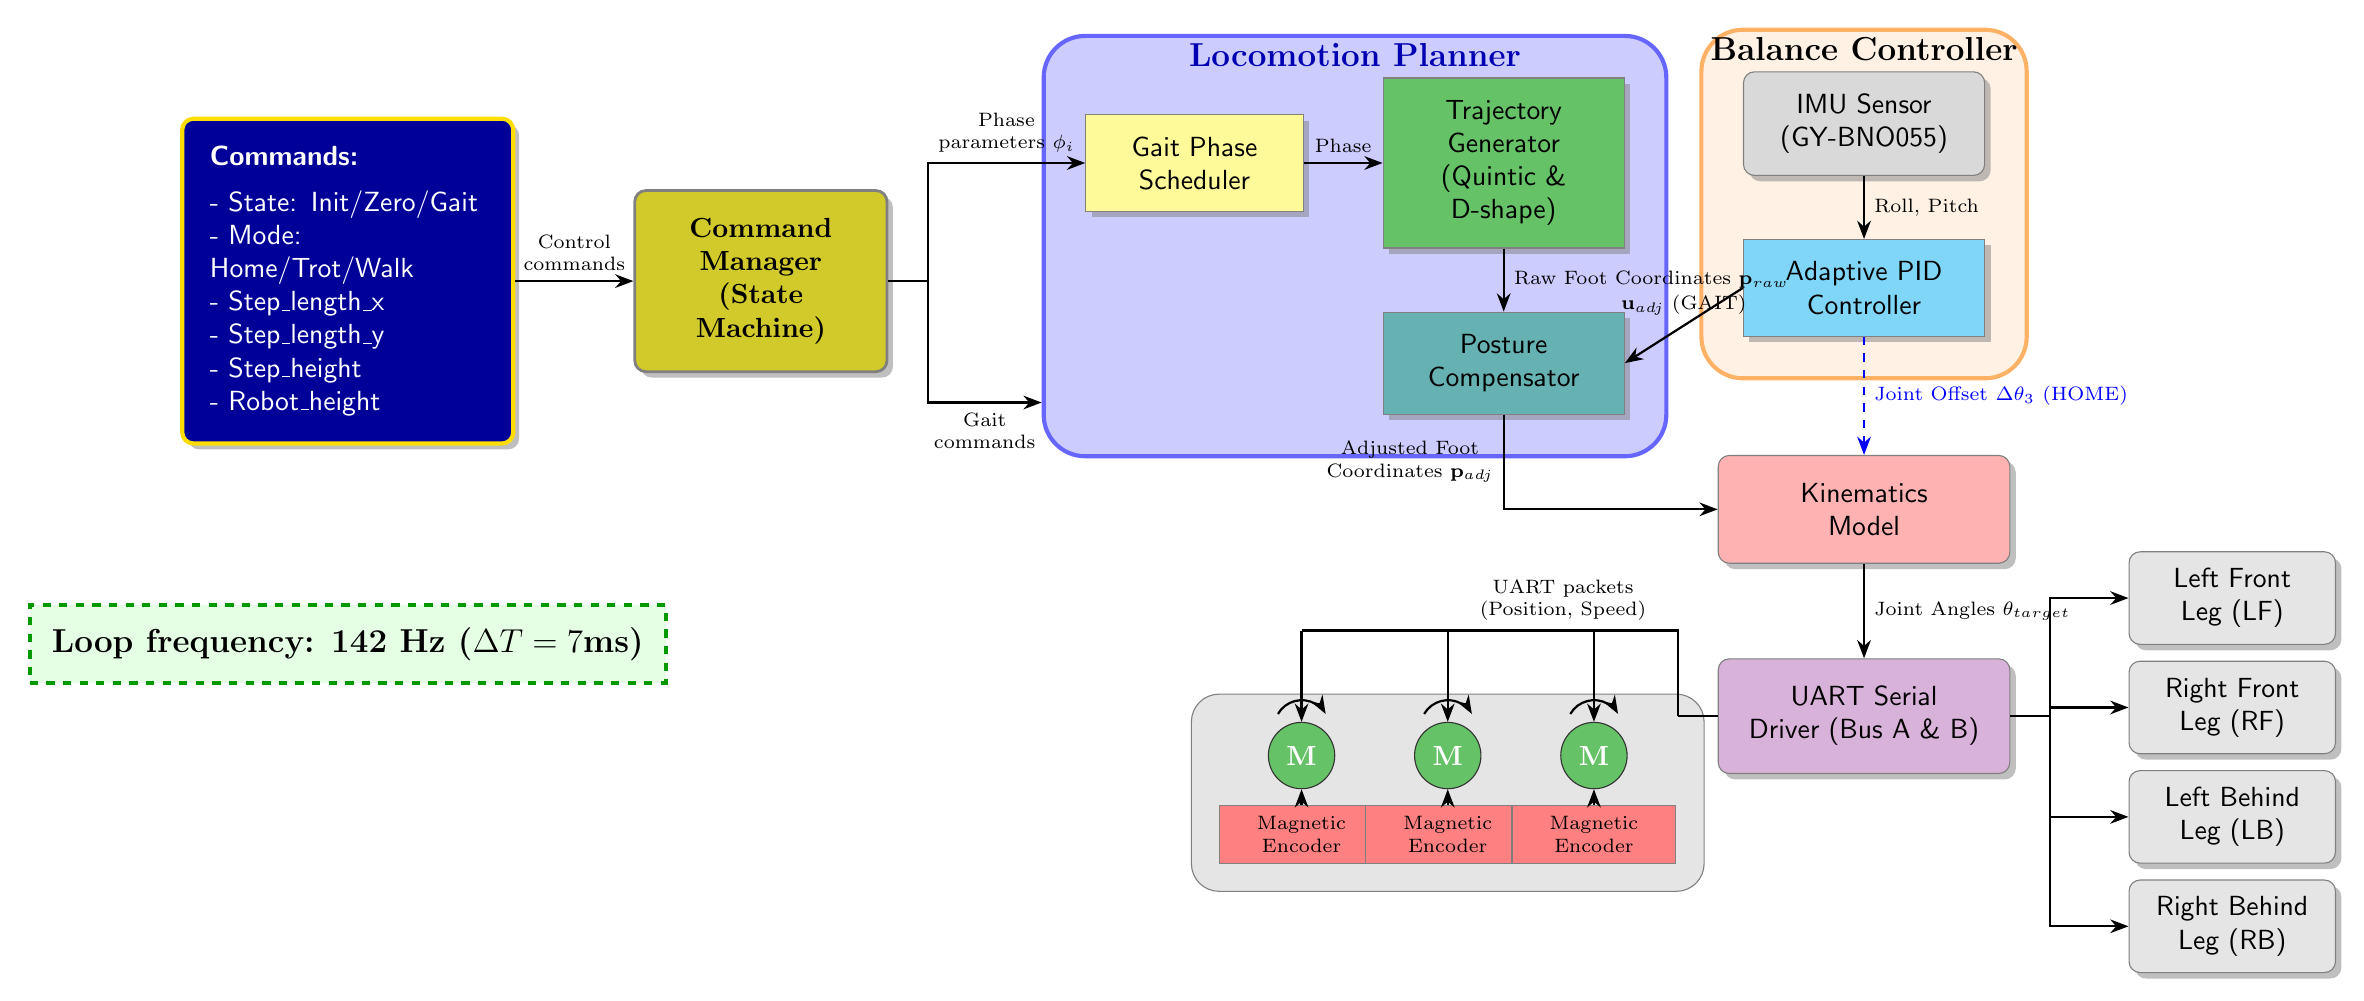
\begin{tikzpicture}[
    font=\sffamily,
    >=Stealth,
    % Styles matching the provided image
    commandbox/.style={rectangle, rounded corners, draw=yellow!80!orange, fill=blue!60!black, text=white, inner sep=10pt, text width=3.5cm, align=left, line width=1.5pt, drop shadow},
    manager/.style={rectangle, rounded corners, draw=black!50, fill=yellow!80!black, inner sep=10pt, text width=2.5cm, align=center, font=\bfseries, line width=1pt, drop shadow},
    plannerbg/.style={rectangle, rounded corners=15pt, draw=blue!60, fill=blue!20, inner sep=15pt, line width=1.5pt},
    balancebg/.style={rectangle, rounded corners=15pt, draw=orange!60, fill=orange!10, inner sep=15pt, line width=1.5pt},
    gaitbox/.style={rectangle, draw=black!50, fill=yellow!40, inner sep=8pt, text width=2.2cm, align=center, drop shadow},
    trajbox/.style={rectangle, draw=black!50, fill=green!60!black!60, inner sep=8pt, text width=2.5cm, align=center, drop shadow},
    posturebox/.style={rectangle, draw=black!50, fill=teal!60, inner sep=8pt, text width=2.5cm, align=center, drop shadow},
    imubox/.style={rectangle, rounded corners, draw=black!50, fill=gray!30, inner sep=8pt, text width=2.5cm, align=center, drop shadow},
    pidbox/.style={rectangle, draw=black!50, fill=cyan!50, inner sep=8pt, text width=2.5cm, align=center, drop shadow},
    ikbox/.style={rectangle, rounded corners, draw=black!50, fill=red!30, inner sep=10pt, text width=3cm, align=center, drop shadow},
    uartbox/.style={rectangle, rounded corners, draw=black!50, fill=violet!30, inner sep=10pt, text width=3cm, align=center, drop shadow},
    legbox/.style={rectangle, rounded corners, draw=black!50, fill=gray!20, inner sep=6pt, text width=2.2cm, align=center, drop shadow},
    freqbox/.style={rectangle, draw=green!60!black, fill=green!10, dashed, inner sep=8pt, font=\bfseries\large, line width=1.5pt},
    motorbg/.style={rectangle, rounded corners=10pt, draw=black!50, fill=gray!20, inner sep=10pt},
    motorcircle/.style={circle, draw=black!80, fill=green!60!black!60, text=white, font=\bfseries, inner sep=4pt},
    sensorbox/.style={rectangle, draw=black!50, fill=red!50, inner sep=4pt, text width=1.8cm, align=center, font=\scriptsize},
    arrowlabel/.style={font=\scriptsize, align=center}
]

% Commands
\node[commandbox] (commands) {
    \textbf{Commands:}\\[1ex]
    - State: Init/Zero/Gait\\
    - Mode: Home/Trot/Walk\\
    - Step\_length\_x\\
    - Step\_length\_y\\
    - Step\_height\\
    - Robot\_height
};

% Command Manager
\node[manager, right=1.5cm of commands] (manager) {Command Manager\\(State Machine)};

% Locomotion Planner
\node[gaitbox, right=2.5cm of manager, yshift=1.5cm] (gait_sel) {Gait Phase\\Scheduler};
\node[trajbox, right=1cm of gait_sel] (traj_gen) {Trajectory\\Generator\\(Quintic \& D-shape)};
\node[posturebox, below=0.8cm of traj_gen] (posture) {Posture\\Compensator};

\begin{scope}[on background layer]
    \node[plannerbg, fit=(gait_sel)(traj_gen)(posture), label={[anchor=north, font=\bfseries\large, text=blue!70!black]north:Locomotion Planner}] (planner) {};
\end{scope}

% Balance Controller
\node[imubox, right=1.5cm of traj_gen, yshift=0.5cm] (imu) {IMU Sensor\\(GY-BNO055)};
\node[pidbox, below=0.8cm of imu] (pid) {Adaptive PID\\Controller};

\begin{scope}[on background layer]
    \node[balancebg, fit=(imu)(pid), label={[anchor=north, font=\bfseries\large, text=black]north:Balance Controller}] (balance) {};
\end{scope}

% Kinematics
\node[ikbox, below=1.5cm of pid] (ik) {Kinematics\\Model};

% UART Driver
\node[uartbox, below=1.2cm of ik] (uart) {UART Serial\\Driver (Bus A \& B)};

% Legs
\node[legbox, right=1.5cm of uart, yshift=1.5cm] (lf) {Left Front Leg (LF)};
\node[legbox, below=0.2cm of lf] (rf) {Right Front Leg (RF)};
\node[legbox, below=0.2cm of rf] (lb) {Left Behind Leg (LB)};
\node[legbox, below=0.2cm of lb] (rb) {Right Behind Leg (RB)};

% Motors Detail
\node[motorcircle, left=3cm of uart, yshift=-0.5cm] (m2) {M};
\node[motorcircle, left=1cm of m2] (m1) {M};
\node[motorcircle, right=1cm of m2] (m3) {M};

\node[sensorbox, below=0.2cm of m1] (s1) {Magnetic\\Encoder};
\node[sensorbox, below=0.2cm of m2] (s2) {Magnetic\\Encoder};
\node[sensorbox, below=0.2cm of m3] (s3) {Magnetic\\Encoder};

\begin{scope}[on background layer]
    \node[motorbg, fit=(m1)(m3)(s1)(s3)] (motor_area) {};
\end{scope}

% Frequency
\node[freqbox, below=2cm of commands] (freq) {Loop frequency: 142 Hz ($\Delta T = 7$ms)};

% Connections
\draw[->, thick] (commands) -- node[above, arrowlabel] {Control\\commands} (manager);

% To Gait Phase Scheduler
\coordinate (split1) at ($(manager.east) + (0.5, 0)$);
\draw[thick] (manager.east) -- (split1);
\draw[->, thick] (split1) |- node[near end, above, arrowlabel] {Phase\\parameters $\phi_i$} (gait_sel.west);
\draw[->, thick] (split1) |- node[near end, below, arrowlabel] {Gait\\commands} ($(planner.west |- posture) + (0, -0.5)$);

\draw[->, thick] (gait_sel) -- node[above, arrowlabel] {Phase} (traj_gen);
\draw[->, thick] (traj_gen) -- node[right, arrowlabel] {Raw Foot Coordinates $\mathbf{p}_{raw}$} (posture);

\draw[->, thick] (imu) -- node[right, arrowlabel] {Roll, Pitch} (pid);

% From PID to Posture Compensator
\draw[->, thick] (pid.west) -- node[above, arrowlabel] {$\mathbf{u}_{adj}$ (GAIT)} (posture.east);

% From Posture to IK
\draw[->, thick] (posture.south) |- node[near start, left, arrowlabel] {Adjusted Foot\\Coordinates $\mathbf{p}_{adj}$} (ik.west);

% From PID to IK directly (HOME Mode)
\draw[->, thick, dashed, blue] (pid.south) -- node[right, arrowlabel, text=blue] {Joint Offset $\Delta\theta_3$ (HOME)} (ik.north);

% From IK to UART
\draw[->, thick] (ik.south) -- node[right, arrowlabel] {Joint Angles $\theta_{target}$} (uart.north);

% UART to Legs
\draw[->, thick] (uart.east) -- ++(0.5,0) |- (lf.west);
\draw[->, thick] (uart.east) -- ++(0.5,0) |- (rf.west);
\draw[->, thick] (uart.east) -- ++(0.5,0) |- (lb.west);
\draw[->, thick] (uart.east) -- ++(0.5,0) |- (rb.west);

% UART to Motors
\coordinate (uart_left) at ($(uart.west) + (-0.5, 0)$);
\coordinate (motor_top) at ($(motor_area.north) + (0, 0.8)$);
\draw[thick] (uart.west) -- (uart_left);
\draw[thick] (uart_left) |- node[near end, above, arrowlabel] {UART packets\\(Position, Speed)} (motor_top);

\draw[->, thick] (motor_top -| m1) -- (m1.north);
\draw[->, thick] (motor_top -| m2) -- (m2.north);
\draw[->, thick] (motor_top -| m3) -- (m3.north);
\draw[thick] (motor_top -| m1) -- (motor_top -| m3);

% Sensors to Motors (feedback)
\draw[->, thick, dashed] (s1) -- (m1);
\draw[->, thick, dashed] (s2) -- (m2);
\draw[->, thick, dashed] (s3) -- (m3);

% Motor rotation arrows
\draw[->, thick] ($(m1.north)+(-0.3,0.1)$) arc[start angle=150, end angle=30, radius=0.35cm];
\draw[->, thick] ($(m2.north)+(-0.3,0.1)$) arc[start angle=150, end angle=30, radius=0.35cm];
\draw[->, thick] ($(m3.north)+(-0.3,0.1)$) arc[start angle=150, end angle=30, radius=0.35cm];

\end{tikzpicture}
\end{document}
